Domain Controllers
\begin{itemize}
    \item Main Functions
    \begin{itemize}
        \item Authenticate users and computers
        \item Deploy Group Policy and scripts
    \end{itemize}
\item Replication and Convergence
\begin{itemize}
    \item Intra-site Replication
    \begin{itemize}
        \item Replication between DCs in same site
        \item Default is immediate
    \end{itemize}
\item Inter-site Replication
\begin{itemize}
    \item Replication between DCs in different sites
    \item Default is 180 minutes
    \item Minimum is 15 minutes
    \item Can be instantly forced by using the 'gpupdate /force' switch
\end{itemize}
\item Inter-site Change Notification
\begin{itemize}
    \item Default is immediate
\end{itemize}
\item CMD: repadmin /replsummary
\end{itemize}
\item Not all DCs are equal
\begin{itemize}
    \item Flexible Single Master Operators (FSMO)
    \begin{itemize}
        \item Relarice ID (RID) Master
        \item PDC Emulator
        \item Infrastructure Master
        \item Domain Naming Master (perforest)
        \item Schema Master (per forest)
    \end{itemize}
\end{itemize}
\end{itemize}

Primary Domain Controller (PDC) Emulator
\begin{itemize}
    \item Password changes performed by other DCs in the domain are replicated preferentially to the PDC emulator.
    \item If a logon authentication fails at a given DC in a domain due to a bad password entered incorrectly, the DC will forward the authentication request to the PDC emulator to validate the request against the most current password. If the PDC reports an invalid password to the DC, the DC will send back a bad password failure message to the requesting user.
    \item Account lockout is processed on the PDC emulator.
    \item Immediate replication to the PDC emulator from another DC
    \begin{itemize}
        \item Lockout of an account
        \item Account is unlocked
        \item Password reset on account
        \item "User Must Change Password at Next Logon" manually set for user
        \item Modification of Local Security Authority (LSA) secret
        \item State changes of the RID Manager
    \end{itemize}
\end{itemize}

Active Directory Security Overview

\textbf{Privileged Accounts}
Includes built-in users and groups with privileges, but also newly created users and groups that are granted privileges.

\textbf{Password Policy}
Either via Group Policy or FGPP the details of the Password Policy need to be configured correctly.

\textbf{Permissions}
Both AD and SYSVOL have permissions that provide granular control, but misconfigured can expose AD to an easy attack.

\textbf{Service Accounts}
Include accounts that are used to support applications, services, scripts, scheduled tasks, and more.

\textbf{Network Protocols}
Backward-compatible network protocols leave the network and AD open for attack. SMB and NTLM need to be secured.

\textbf{Trusts}
Domain and Forest trusts have many caveats and configurations that often go misconfigured and open to attack.

\textbf{AD Processes}
Processes such as SDProp, Kerberos authentication, and Kerberos ticketing need to be secured.

\textbf{User Attributes}
Controls such as SPNs, Kerberos delegation, Primary Group ID, SIDHistory, and more, need to be secured.

\textbf{Unsecure Users}
These accounts are those that have not logged or changed their password for quite some time, as well as those with non-expiring passwords.

\textbf{User Rights}
Each domain controller has special privileges that can grant power over the server and even the entire AD infrastructure.

\textbf{AAD Connections}
Settings within the on-prem AD that allow for communications and synchronization with Azure AD need to be secured.

\textbf{Computer Attributes}
Kerberos delegations and group memberships can provide an unmonitored attack surface and every attacker looks for these.

The Windows Security Model

\begin{itemize}
    \item Security Identifiers (SIDs)
    \item Tokens
    \item Object-based Access Control
    \item User Authentication
\end{itemize}

SIDS
\begin{itemize}
    \item User and computer account = 1 single object in AD
    \begin{itemize}
        \item A user / computer account only exists one time in AD
        \item User / computer accounts can have memberships in many groups
    \end{itemize}
\item Security Identifiers (SIDs)
\begin{itemize}
    \item Users
    \item Groups
    \item Computers
\end{itemize}
\item PowerShell:
\begin{itemize}
    \item \texttt{Get-aduser nina -properties sid}

\end{itemize}
\end{itemize}

\begin{figure}
    \centering
    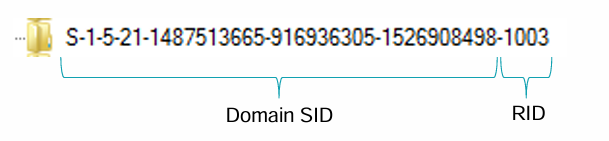
\includegraphics[width=0.75\linewidth]{sid.png}
    \caption{Security Identifiers (SIDs)}
    \label{fig:placeholder}
\end{figure}

Authentication Tokens
\begin{itemize}
    \item Given out by Domain Controller at user logon
    \item Contents
    \begin{itemize}
        \item User SID
        \item Group SIDs
        \item Privileges
        \item CMD:
        \begin{itemize}
            \item \texttt{whoami /all}
        \end{itemize}
    \item Only refreshed with user logged off or upon computer restart
    \end{itemize}
\end{itemize}

Object-based Access Control
\begin{itemize}
    \item ACL-Access Control List-Security tab
    \begin{itemize}
        \item Associated with Windows security objects
        \item Entries can include: users, groups, computers
        \item Defines the access per security principal
        \item ACL is list of SIDs
        \begin{itemize}
            \item GUI translates
            \item Orphaned SIDs
        \end{itemize}
    \end{itemize}
\item Objects with ACLs
\begin{itemize}
    \item Files and Folders
    \item Registry Keys
    \item Printers
    \item AD Objects
    \item Services
\end{itemize}
\end{itemize}

\begin{figure}
    \centering
    
    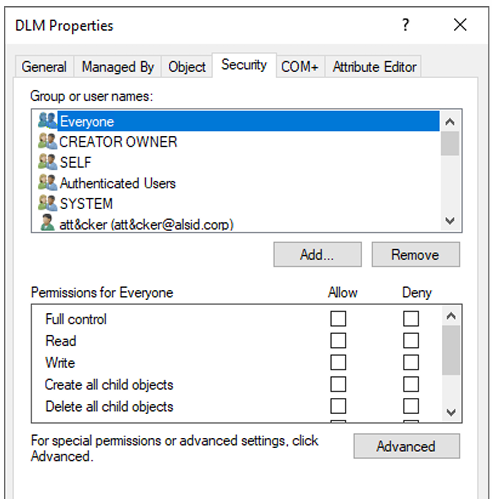
\includegraphics[width=0.75\linewidth]{acl.png}
    \caption{Access Control List (ACL)}
    \label{fig:placeholder}
\end{figure}

User Authentication

\begin{figure}
    \centering
    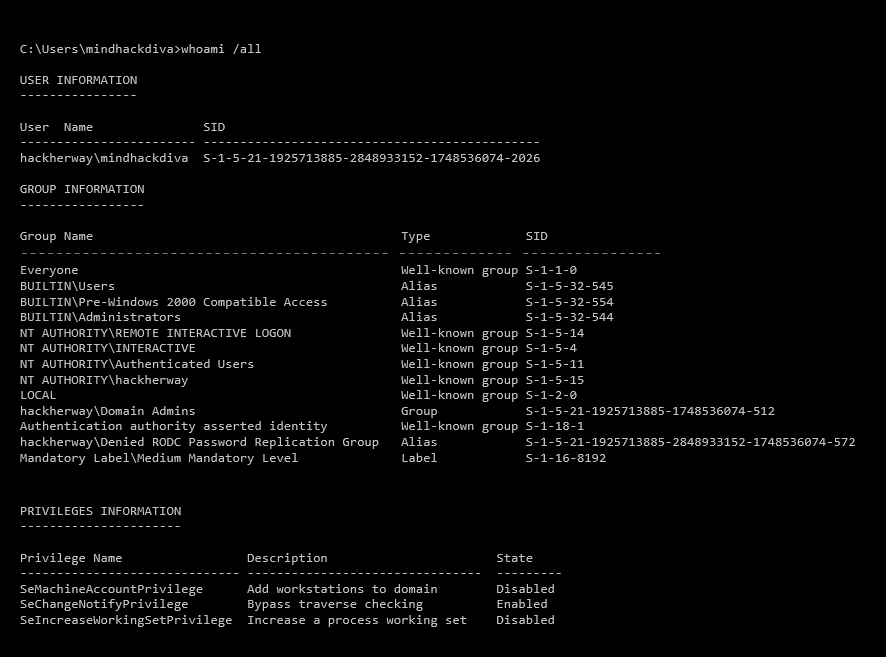
\includegraphics[width=0.75\linewidth]{whoamicmd.png}
    \caption{whoami command}
\end{figure}

\begin{figure}
    \centering
    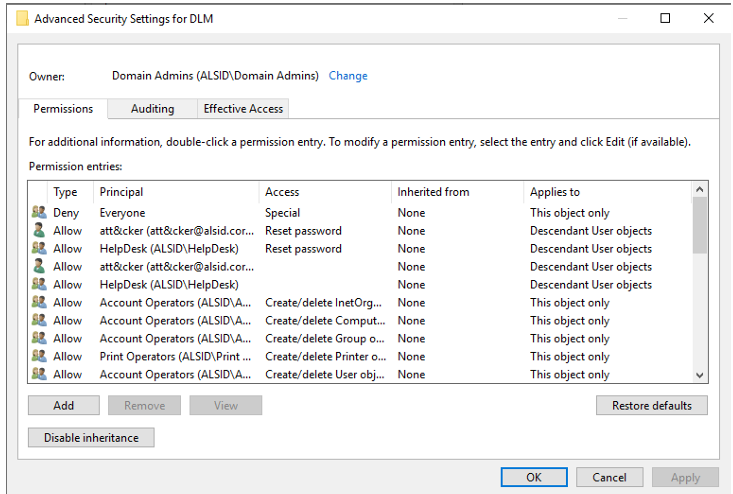
\includegraphics[width=0.75\linewidth]{dlm.png}
    \caption{DLM}
    \label{fig:placeholder}
\end{figure}

